\chapter{Phase plane analysis}\label{Phase plane analysis}
In the last chapter we considered ODE systems with only a single steady state. Even though we are going to restrict ourselves to a two-dimensional ODE systems, such systems can have many non-trivial steady states. We need to be able to combine such information to give an idea of what the global dynamics will be, even though we only have local analysis. 

This will be a graphical method and in some ways provides a two-dimensional extension to the methods seen in \chap{Stationary states and stability}. Specifically, in \chap{Stationary states and stability} we could understand the entire dynamics of the system in the $(u,\dot{u})$ plane, when we have two variables, we consider the $(u,v)$ plane instead, which is known as a `phase plane'. To construct a phase plane, instead of considering a single trajectory as in the $(t,u)$ simulation, we consider the motion of a trajectory across all points in the $(u,v)$ space. To aid in our understanding we introduce a new concept.

\begin{defin}
Consider an ODE system
\bb
\dot{\bm{u}}=\bm{F}(\bm{u}),
\ee
where $\bm{F}(\bm{u})=(F_1(u_1,\dots,u_n),\dots,F_n(u_1,\dots,u_n))$. The nullclines are the curves defined by
\bb
F_i(u_1,\dots,u_n)=0,
\ee
for all $i=1,\dots,n$.
\end{defin}
Nullclines are a useful concept because on each separate curve the dynamics of at least one variable is stationary, thus, the direction across a nullcline is simplified. Moreover, if all nullclines meet at a given point all dynamics must be stationary, \ie by definition all nullclines meet at steady states.
\begin{example}[frametitle=Nullclines]\label{Nullcline_example_example}
Consider the system
\begin{align}
\dot{u}&=v-(u-2)(u-3),\label{Nullcline_1}\\
\dot{v}&=v-\ln(u),\label{Nullcline_2}
\end{align}
in the half plane $u>0$.

\COL{The steady states of this would satisfy
\bb
\ln(u)=(u-2)(u-3),
\ee
which has no closed form solution. We could estimate the solutions using a numerical root finding }\COL{algorithm. However, by plotting the nullclines,
\begin{align}
v&=(u-2)(u-3),\\
v&=\ln(u),
\end{align}
in \fig{Nullcline_example}, we immediately  see there are exactly two steady states.}
\end{example}
\begin{figure}[!!!h!!!tb]
\centering
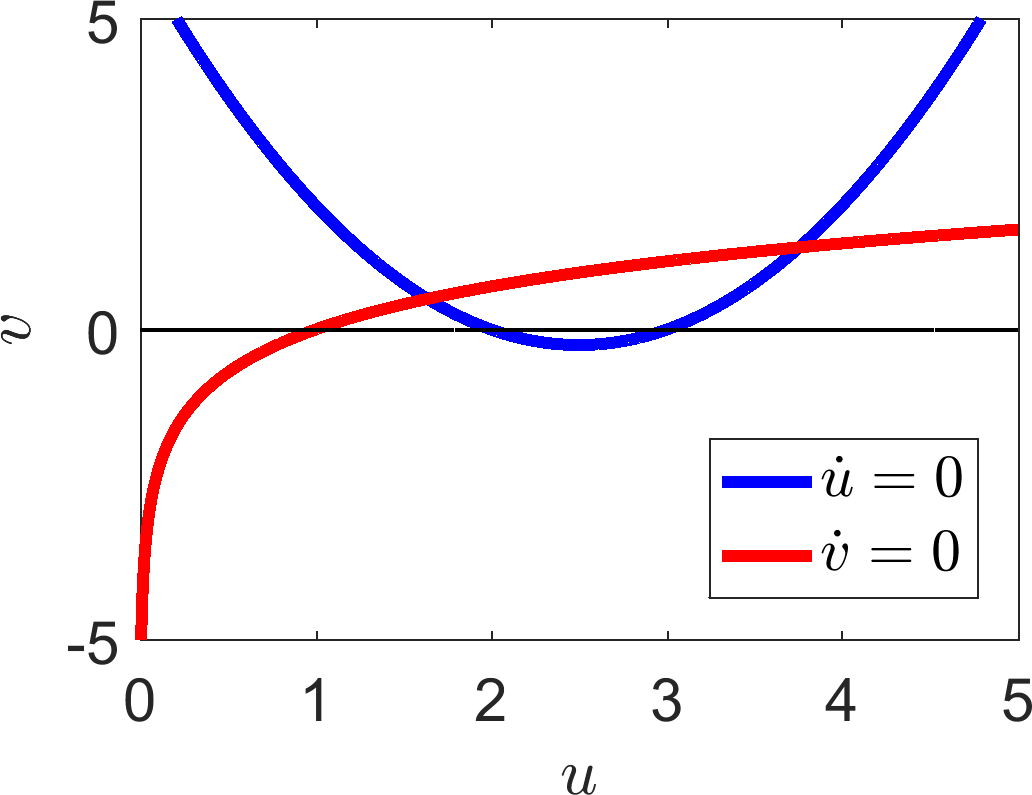
\includegraphics[width=\ttp]{../Pictures/Nullcline_example.png}
\caption{\label{Nullcline_example}Plot of the nullclines of \eqns{Nullcline_1}{Nullcline_2}.}
\end{figure}

Consider a general nullcline, for example $\dot{u}=0$. This line must delineate the regions where the derivative is positive and negative. Namely, on one side of the line $\dot{u}>0$, whilst on the other $\dot{u}<0$. The same can be said of the $\dot{v}=0$. Thus, the nullclines segment the $(u,v)$ into regions of different dynamics. We return to example \ref{Nullcline_example_example} with this knowledge and specify the signs of the derivatives in each region.
\begin{example}[frametitle=Derivative signs]\label{Nullcline_signs}
\COL{We first consider the $\dot{u}$ nullcline
\bb
v=(u-2)(u-3),
\ee
illustrated in \fig{u_nullcline}. Pick any point vertically higher than than the curve, \eg (2,10), and consider the sign of \eqn{Nullcline_1}. Specifically, substituting this value in we get
\bb
\dot{u}=10>0.
\ee
Thus, above the curve $\dot{u}>0$ and $\dot{u}<0$ below the curve \see{u_nullcline}. Once, we know the sign of the derivative in each section we can draw arrows to illustrate the local direction in which the trajectory will be heading. For example, in a region with $\dot{u}>0$ the $u$ coordinate will be increasing and, so the arrowhead points to the right \ie increasing $u$ direction.

We can do the same for the $v$ regions. For example, consider the point $(5,0)$,
\bb
\dot{v}=0-\ln(5)<0.
\ee
Hence, to the right of the $v$ nullcline $v$ is decreasing. By a similar process $v$ is increasing to the left of the $v$ nullcline \see{v_nullcline}.

We now combine this information in each region providing a sketch of how a trajectory will act anywhere in the plane. In addition we add arrows the nullclines where we remember that }\COL{there is no movement in the $u$ direction on the $u$ nullcline and no movement in the $v$ direction along the $v$ nullcline. Namely, the arrows are vertical and horizontal on the $u$ and $v$ nullclines, respectively. Equally, we pay explicit attention to which way these arrows are directed according to the surrounding information.

All of this information is plotted in \fig{uv_nullcline}. Critically, in this case we are able to suggest what forms the steady states will have. The steady state on the left (approximately (1.6,0.5)) will be unstable because all of the arrows near to the steady state point away from the steady state. The steady state on the right (approximately, (3.8,1.3)) appears to be a saddle as arrows in the horizontal direction point towards the steady state, whilst arrows in the vertical direction point away from the state.

However, to ensure we are right we have to run the analysis. We will not do this here because the algebra gets very hairy and, as mentioned, you would need to use a numerical root finder to estimate the steady states to substitute into the Jacobian. If we do do this numerically we find that the eigenvalues of the left steady state are $\lambda_\pm\approx 1.36\pm0.69I$, thus, the point is indeed unstable, but an unstable spiral, which we could not have predicted from the graph. The eigenvalues for the steady state on the right are $\lambda_-\approx -2.43<0<0.92=\lambda_+$, hence the point is a saddle, justifying our diagram.}
\end{example}

From this example we have seen that phase planes are helpful diagrams, which encapsulate lots of stability information. However, as illustrated in comparing the diagram with the actual analytical values of the eigenvalues it can be difficult to tell the difference between (un)stable nodes and (un)stable spirals. Equally, as we saw in the last chapter, sketches only provide the correct insight if you draw the system correctly. If there had been a parameter in this system that we could vary then there may have been a stability case, dependent on the parameter, that we would miss if we had only drawn one diagram. Thus, a phase plane should always be backed up with linear analysis. The linear analysis provides the local information, whilst the phase plane allows us to approximately see how all the dynamics fit together.
%\begin{figure}[!!!h!!!tb]
%\centering
%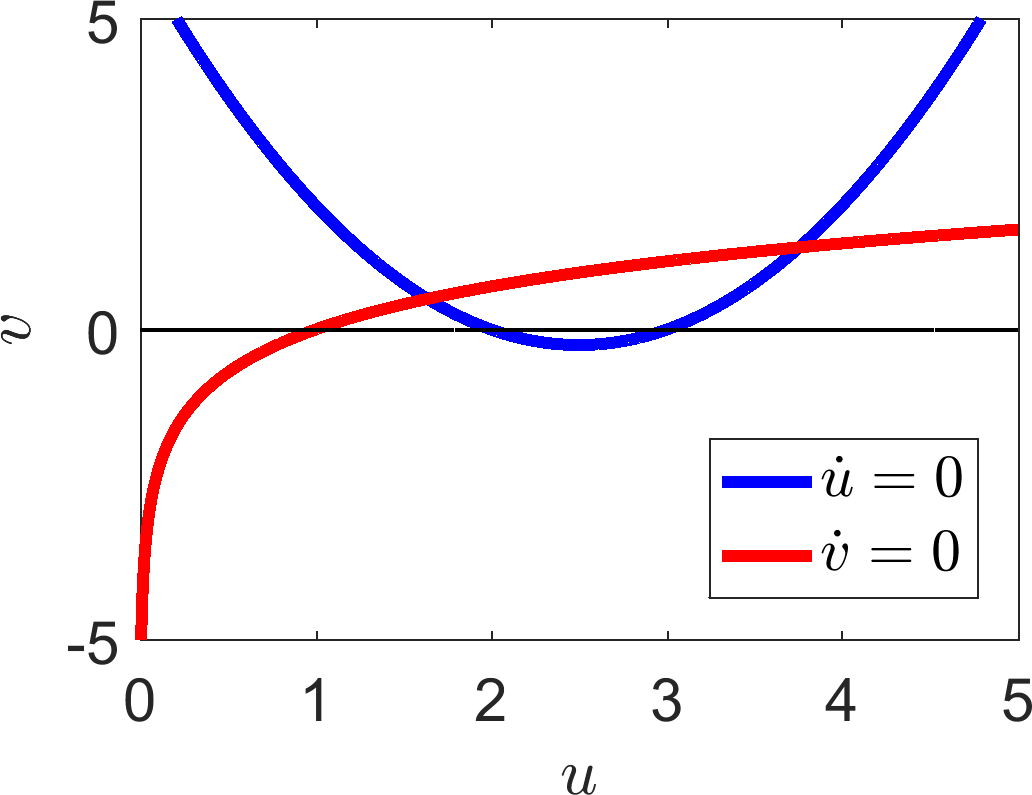
\includegraphics[width=\ttp]{../Pictures/Nullcline_example.png}
%\caption{\label{Nullcline_example}Plot of the nullclines of \eqns{Nullcline_1}{Nullcline_2}.}
%\end{figure}
\begin{figure}[!!!h!!!tbp]
\centering
\subfigure[\label{u_nullcline}]{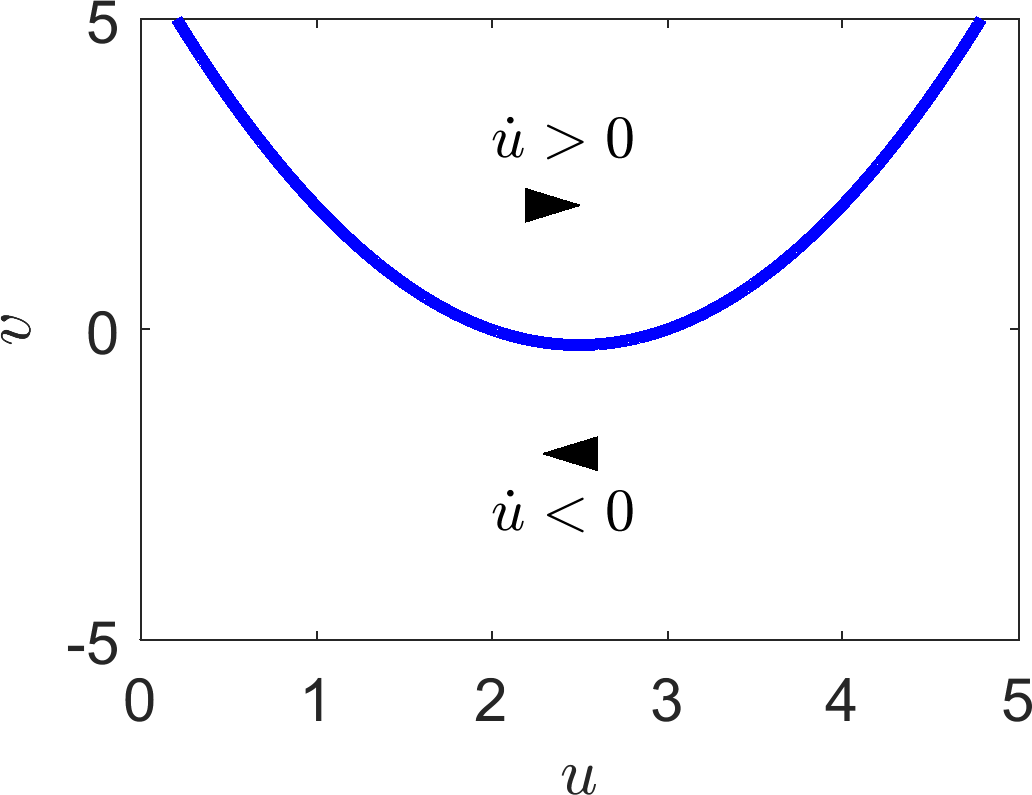
\includegraphics[width=\ttp]{../Pictures/u_nullcline.png}}
\subfigure[\label{v_nullcline}]{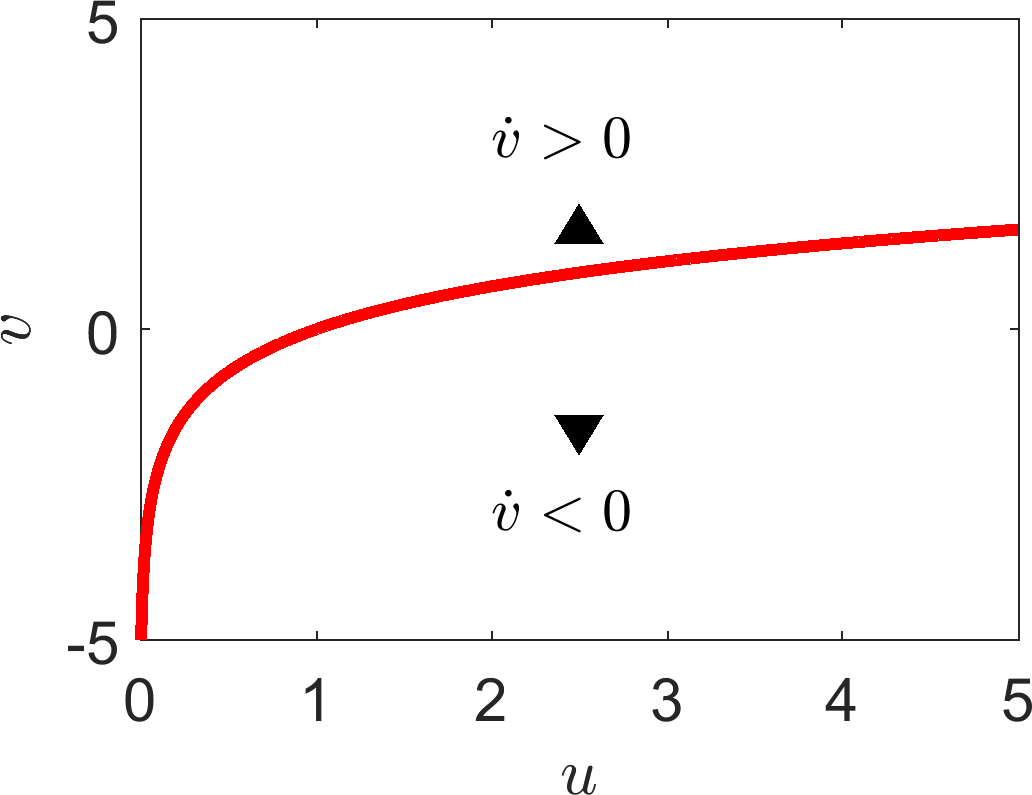
\includegraphics[width=\ttp]{../Pictures/v_nullcline.png}}
\subfigure[\label{uv_nullcline}]{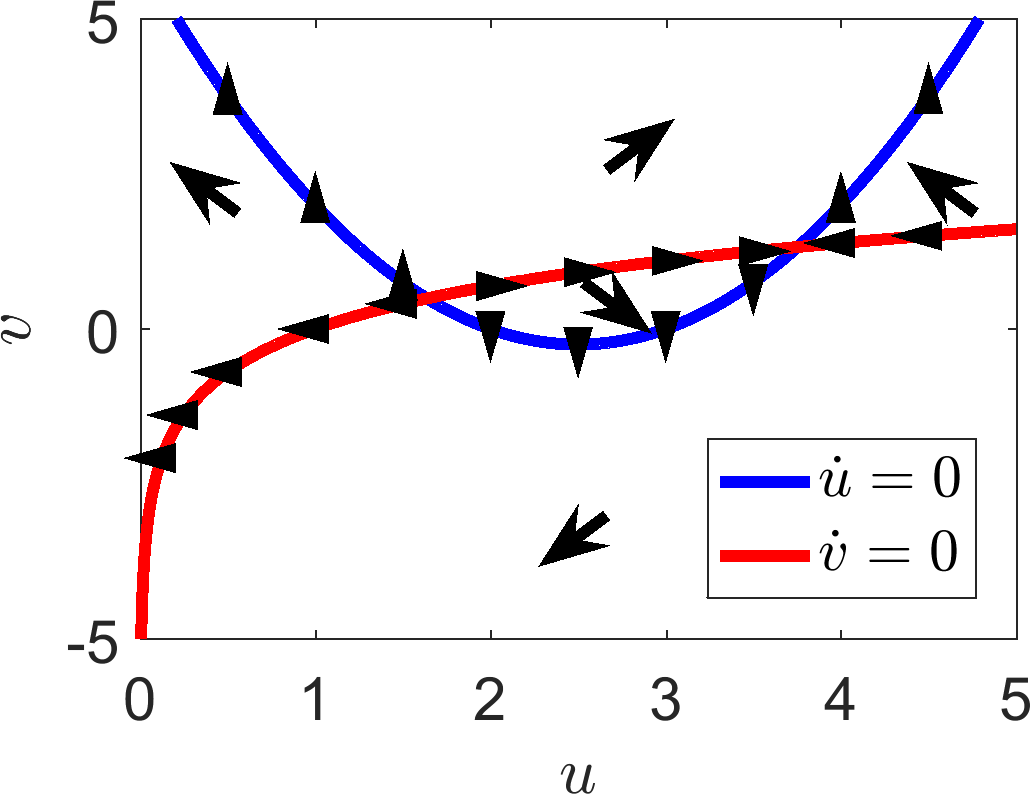
\includegraphics[width=\ttp]{../Pictures/uv_nullcline.png}}
\subfigure[\label{Phase_plane_example}]{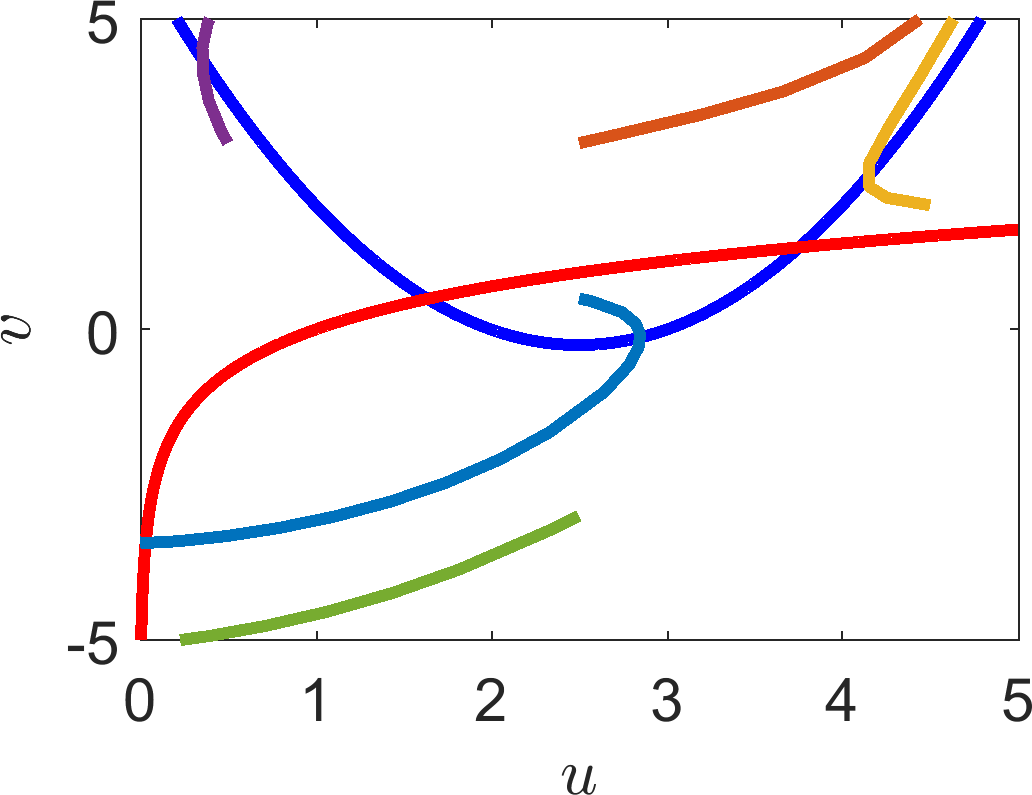
\includegraphics[width=\ttp]{../Pictures/Phase_plane_example.png}}
\caption{\label{Derivative_signs}Specifying the signs of the derivatives on either side of the (a) $\dot{u}$ and (b) $\dot{v}$ nullcline. The arrowheads indicate the general direction that a trajectory will be heading. These results can then be combined into the direction plots seen in (c). Finally, in (d), we simulate a number of trajectories, which demonstrate that the arrows in (c) provide the correct general idea.}
\end{figure}


%\begin{example}[frametitle=Failure]
%As mentioned not all balances are valid, which is what we will seen in this example%Consider the following ODE system
%\begin{align}
%  \tikzmark{a}\dot{u}=k_0\tikzmark{b}+k_1\tikzmark{c}u-k_2uv, \quad u(0)=u_0,\label{Non-dim_9}\\
% \nonumber \\
%    \tikzmark{e}\dot{v}=k_3\tikzmark{f}+k_4\tikzmark{g}v-k_2uv, \quad v(0)=v_0.\label{Non-dim_10}
%\tikz[overlay,remember picture]
%{\draw[square arrow1] (a.south) to (b.south);}
%\tikz[overlay,remember picture]
%{\draw[square arrow1] (b.south) to (c.south);}
%\tikz[overlay,remember picture]
%{\draw[square arrow1] (e.south) to (g.south);}
%%\end{align}
%There are three variables $u$, $v$ and $t$ and so we need three balances. The chosen balances are illustrated on the equations using arrows. Extracting information from the balances we find that
%\bb
%\frac{[u]}{[t]}=k_0=k_1[u], \quad \frac{[v]}{[t]}=k_4[v].
%\ee
%From this point we quickly discover that
%\bb
%[t]=\frac{1}{k_1} \textrm{ and } [t]=\frac{1}{k_4}.
%\ee
%Since, generally, $k_1\neq k_4$ we cannot satisfy both balances, thus, we must consider a different non-dimensionalisation.
%
%One possible valid non-dimensionalisation is
%\begin{align}
%  \tikzmark{a}\dot{u}=k_0\tikzmark{b}+k_1\tikzmark{c}u-k_2uv, \quad u(0)=u_0,\nonumber\\
% \nonumber \\
%    \tikzmark{e}\dot{v}=k_3\tikzmark{f}+k_4\tikzmark{g}v-k_2uv, \quad v(0)=v_0.\nonumber
%\tikz[overlay,remember picture]
%{\draw[square arrow1] (a.south) to (b.south);}
%\tikz[overlay,remember picture]
%{\draw[square arrow1] (b.south) to (c.south);}
%\tikz[overlay,remember picture]
%{\draw[square arrow1] (e.south) to (f.south);}
%\end{align}
%See your problem sheets for details.
%\end{example}


%\begin{figure}[!!!h!!!tb]
%\centering
%\subfigure[\label{IC_0.1}]{\includegraphics[width=\ttp]{../Pictures/Comparing_pendulums_IC_1.png}}
%\subfigure[\label{IC_1}]{\includegraphics[width=\ttp]{../Pictures/Comparing_pendulums_IC_10.png}}
%\caption{\label{Different_ICs}Comparing \eqns{Spring_eqn}{Bob_eqn} with initial conditions (a) $y=0=\theta$ and (b) $y=1=\theta$. Parameter values $r=g=k=m=1$.}
%\end{figure}
%
%
%\begin{example}[frametitle=Zombies]\label{Zombies}
%Humans, $H$ and zombies, $Z$ interact through the following three interactions \see{Zombie_picture}]:
%\end{example}
%\begin{figure}[!!!h!!!tb]
%\centering
%\includegraphics[width=\tp]{../Pictures/Zombies.png}
%\caption{\label{Zombie_picture} Possible outcomes of human-zombie interactions.}
%\end{figure}

\section{Check list}
By the end of this chapter you should be able to:
\begin{todolist}
\item define what a nullcline is;
\item understand the relationship between steady states and the points at which nullclines cross;
\item plot nullclines;
\item sketch arrows showing general trajectory directions on the phase plane;
\item interpret the stability of the steady states from the information plotted on a phase plane.
\end{todolist}





